
\documentclass[12pt,aspectratio=169]{beamer}

\input{style.tex}
\usepackage{xcolor,colortbl}

% Wide frame
\newcommand\Wider[2][3em]{%
	\makebox[\linewidth][c]{%
		\begin{minipage}{\dimexpr\textwidth+#1\relax}
			\raggedright#2
		\end{minipage}%
	}%
}

% Math symbols
\DeclareMathSymbol{\R}{\mathalpha}{AMSb}{"52}
\newcommand{\boldbeta}{\ensuremath{\boldsymbol{\beta}}}
\newcommand{\binaryspace}{\ensuremath{\left\{ -1, +1 \right\}}}

% Argmin and argmax
\DeclareMathOperator{\Tr}{Tr}

% L2 norm
\newcommand{\norm}[2][2]{\left\lVert #2 \right\rVert_{#1}}

\begin{document}

	{\usebackgroundtemplate{\tikz\node[opacity=0.4,inner sep=0]{
\includegraphics[width=\paperwidth,height=\paperheight]{images/header}};}%
	\begin{frame}[plain]
		\vspace{0.5cm}
		\title{\large \begin{spacing}{1.0}Fondamenti di Machine Learning\end{spacing}\vspace{0.25em}
			\normalsize \begin{spacing}{1.0}\textbf{Laurea Triennale in Ingegneria delle Comunicazioni}\end{spacing}\vspace{0.5em}}
		\subtitle{\Large \textbf{6: Data preprocessing, model selection, model evaluation}}
		\date{
			{
\includegraphics[scale=0.8]{images/Uniroma1}}
		}
		\author{
			\setlength{\tabcolsep}{2pt}
			\begin{tabular}{rl}
				\textbf{Lecturer}: & S. Scardapane \\
			\end{tabular}
		}\titlepage
	\end{frame}
	}

\part{1}

\section{Data preprocessing}

\subsection{Feature normalization}

\begin{frame}{Normalizzazione delle feature (1)}
	
	Consideriamo dei clienti di una banca, descritti da due feature:
	%
	\begin{itemize}
		\item \textbf{Sesso}, codificato come $\left[0, 1\right]$ (maschio) o $\left[1,0\right]$ (femmina).
		\item \textbf{Reddito} [\$/mese], che varia da 0 a $10.000$.
	\end{itemize}
	%
	Ora consideriamo un cliente $\vc{x} \in \R^3$, e due altri clienti molto simili a $\vc{x}$ (ricordando che $\lVert \mathbf{x} \rVert = \sqrt{\sum_i x_i^2}$):
	%
	\begin{itemize}
		\item $\vc{x}'$ è identico a $\vc{x}$, ma di sesso opposto. Abbiamo che $\lVert \vc{x}' - \vc{x}\rVert = \sqrt{2}$.
		\item $\vc{x}''$ è identico a $\vc{x}$, ma il suo reddito mensile è superiore di $100$. Abbiamo che $\lVert\vc{x}'' - \vc{x}\rVert = 100$.
	\end{itemize}
	
\end{frame}

\begin{frame}{Normalizzazione delle feature (1)}
	
	Qualsiasi algoritmo basato sulla distanza Euclidea tra i modelli (ad esempio, $k$-NN) darà $10$ volte più importanza al reddito rispetto al sesso, \textit{indipendentemente dalla sua effettiva importanza per il task di classificazione}.
	
	In pratica, quasi qualsiasi algoritmo di machine learning non funzionerà correttamente se le feature sono misurate in unità con scale molto diverse.
	
	Il processo di trasformazione dei dati (preprocessing) per fare sì che tutte le feature si trovino nello stesso range si chiama \textbf{normalizzazione delle feature} (\myalert{feature normalization}).
	
\end{frame}

\begin{frame}{Normalizzazione min-max}

	Nella \textbf{normalizzazione min-max}, ridimensioniamo ogni feature nell'intervallo $\left[0,1\right]$:
	%
	$$
	x_i = \frac{x_i - x_{i, \text{min}}}{x_{i, \text{max}} - x_{i, \text{min}}} \,.
	$$
	%
	dove $x_{i, \text{min}}$ ($x_{i, \text{max}}$) sono rispettivamente il valore minimo e massimo per la $i$-esima feature calcolati sull'intero dataset. Possiamo successivamente mappare su un intervallo generico $\left[\alpha, \beta\right]$ applicando una seconda trasformazione:
	%
	$$
	x_i = (\beta - \alpha)x_i + \alpha \,.
	$$
	
\end{frame}

\begin{frame}{Robust and standard scaling}
	
	Un'altra tecnica molto usata è la \textbf{normalizzazione standard}:
	%
	$$
	x_i = \frac{x_i - \mu_i}{\sigma_i^2} \,.
	$$
	%
	dove $\mu_i$ è la media empirica e $\sigma_i^2$ la varianza empirica, sempre calcolate sull'intero dataset.
	
	La maggior parte delle tecniche di normalizzazione può essere applicata escludendo i dati `estremi' dal calcolo delle statistiche (ad esempio, utilizzando solo i dati tra il $15$° e l'$85$° percentile) per fornire maggiore robustezza ai valori anomali. A volte, questo viene chiamato \textbf{normalizzazione robusta}.
	
\end{frame}

\begin{whiteframe}{Un esempio di normalizzazione delle caratteristiche}
	
	\Wider{
		\begin{figure}
			\centering
			\footnotesize
			\subfloat[Normalizzazione min-max]{
				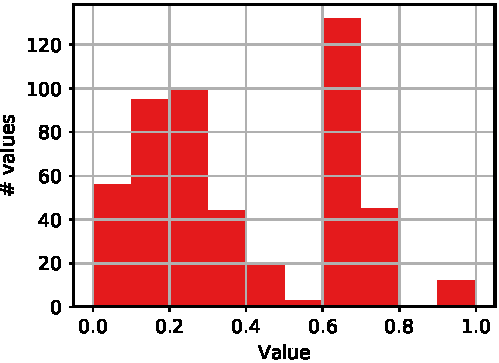
\includegraphics[width=3.5cm,keepaspectratio]{../scripts/feature_normalization_minmax.pdf} %
			}\hfil
			\subfloat[Normalizzazione standard]{
				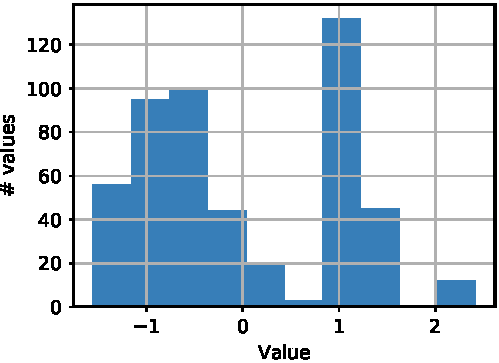
\includegraphics[width=3.5cm,keepaspectratio]{../scripts/feature_normalization_normal.pdf} %
			}\hfil
			\subfloat[Normalizzazione robusta]{
				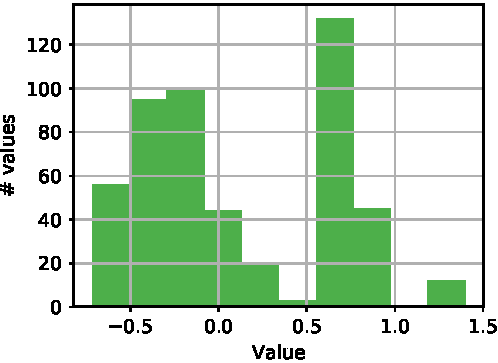
\includegraphics[width=3.5cm,keepaspectratio]{../scripts/feature_normalization_robust.pdf} %
			}\vfil
			\caption{Un confronto tra diverse tecniche di normalizzazione delle feature sulla terza feature del dataset Boston. La distribuzione dei dati non viene mai influenzata. La normalizzazione robusta viene calcolata sull'intervallo interquartile (cioè, tra il $25$° e il $75$° percentile).}
			
		\end{figure}
	}
\end{whiteframe}

\begin{frame}{Normalizzazione logaritmica}
	
	Molte caratteristiche nel mondo reale presentano distribuzioni fortemente asimmetriche con una coda molto lunga. Un esempio classico è il reddito di una persona.
	
	Una normalizzazione comune in questo caso è la \textbf{normalizzazione logaritmica}:
	$$
	x_i = \log(x_i) \,.
	$$
	%
	La normalizzazione logaritmica è importante quando ci interessano solo i cambiamenti relativi in una quantità. Ad esempio, l'aumento relativo di $a+1$ rispetto a $a$ è sempre $\log(1)$ utilizzando la normalizzazione logaritmica, indipendentemente dal valore di $a$.
	
\end{frame}

\begin{whiteframe}{Un esempio di normalizzazione logaritmica}
	
	\begin{figure}
		\centering
		\subfloat[Distribuzione originale]{
			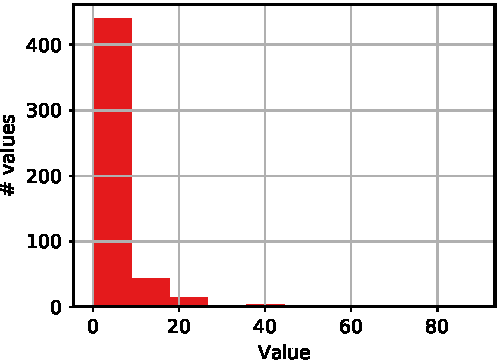
\includegraphics[width=4.5cm,keepaspectratio]{../scripts/log_normalization_original.pdf} %
		}\hfil
		\subfloat[Dopo la normalizzazione logaritmica]{
			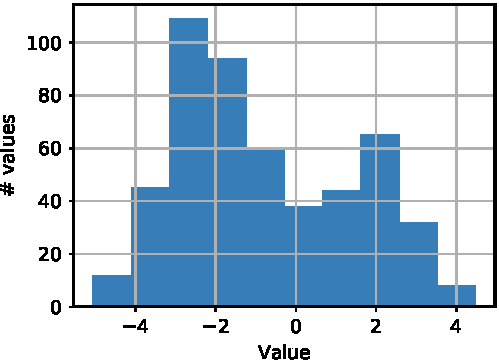
\includegraphics[width=4.5cm,keepaspectratio]{../scripts/log_normalization_transformed.pdf} %
		}\vfil
		\caption{Normalizzazione logaritmica applicata alla prima feature del dataset Boston (tasso di criminalità).}
	\end{figure}
	
\end{whiteframe}

\subsection{Imputazione dei dati mancanti}

\begin{frame}{Il problema dei dati mancanti}
	
	Un altro problema comune sono i \myalert{dati mancanti} (\myalert{missing feature}), in cui elementi della matrice di input $\vc{X}$ sono mancanti. La maggior parte dei metodi di apprendimento non è in grado di gestire i dati mancanti senza una forma di pre-processing.
	
	Una strategia di base è rimuovere qualsiasi riga con una o più caratteristiche mancanti. Questo approccio può essere sub-ottimale per due motivi:
	%
	\begin{enumerate}
		\item Se molte feature hanno valori mancanti, possiamo ottenere un dataset estremamente ridotto.
		\item Se la mancanza di dati è correlata con qualche fattore sottostante (ad esempio, gli utenti maschi sono più riluttanti a condividere alcune informazioni), allora il dataset risultante sarà sbilanciato.
	\end{enumerate}
	
\end{frame}

\begin{frame}{Imputazione della media e della mediana}
	
	Un approccio efficace nella pratica è sostituire i dati mancanti con la media (o mediana) calcolata rispetto alla colonna corrispondente.
	
	Per i problemi di classificazione, possiamo anche fare \textbf{imputazione condizionale dei dati}, dove la media (o mediana) è calcolata utilizzando solo i dati della classe corrispondente.
	
	Se abbiamo conoscenze preliminari sul \textit{come} mancano i dati, possiamo fare un'imputazione condizionale rispetto ad altre caratteristiche di input, ad esempio, calcolare la media rispetto alla nazionalità dell'utente.
	
\end{frame}

\begin{frame}{Variabili indicatrici per i dati mancanti}
	
	\begin{itemize}
		\item Se una variabile categorica ha valori mancanti, un approccio alternativo è aggiungere una nuova categoria corrispondente al caso mancante. Ad esempio, considerando una caratteristica $x = \left\{ \text{maschio}, \text{femmina} \right\}$:
		$$
		\text{male} = \begin{bmatrix}
			1 \\ 0 \\ 0
		\end{bmatrix} \,, \,\,
		\text{female} = \begin{bmatrix}
			0 \\ 1 \\ 0
		\end{bmatrix} \,, \,\,
		\text{missing value} = \begin{bmatrix}
			0 \\ 0 \\ 1
		\end{bmatrix} \,.
		$$
		%
		\item Lo stesso può essere fatto con una variabile continua; in quel caso, usiamo un valore predefinito per la feature quando manca e aggiungiamo una feature che è $1$ se la feature manca, $0$ altrimenti.
	\end{itemize}
	
\end{frame}

\begin{frame}{Imputazione come problema di apprendimento}
	
	Supponiamo che solo la $k$-esima feature abbia valori mancanti. Possiamo modellare l'imputazione dei dati mancanti come un problema di apprendimento supervisionato:
	%
	$$
	f(\vc{x}_{-k}, y) = x_k \,,
	$$
	%
	dove $\vc{x}_{-k}$ denota l'insieme di tutte le feature escludendo la $k$-esima. L'imputazione della media e della mediana sono un caso speciale, dove l'output di $f$ è costante (o costante a tratti per l'imputazione condizionale).
	
	È raro ottenere buoni risultati con modelli eccessivamente complicati per $f$. La regressione lineare (o regressione logistica) sono scelte comuni.
	
\end{frame}

\section{Selezione del modello}

\subsection{K-fold cross-validation}

\begin{frame}{K-fold cross-validation}
	
	Fino ad ora, abbiamo utilizzato la procedura di holdout per stimare il possibile overfitting. Un singolo holdout può essere fuorviante, in particolare per dataset di medie dimensioni (alta varianza).
	
	Un modo più comune per valutare i modelli è eseguire una \myalert{k-fold cross-validation}:
	
	\begin{enumerate}
		\item Dividiamo il dataset in $k$ parti di uguale dimensione $\mathcal{S}_1, \ldots, \mathcal{S}_k$.
		\item Alleniamo su $\mathcal{S}_2, \ldots, \mathcal{S}_k$, e testiamo su $\mathcal{S}_1$. Otteniamo un errore $E_1$.
		\item Alleniamo su $\mathcal{S}_1, \mathcal{S}_3, \ldots, \mathcal{S}_k$, e testiamo su $\mathcal{S}_2$. Ottieniamo un errore $E_2$.
		\item ...
		\item Alleniamo su $\mathcal{S}_1, \ldots, \mathcal{S}_{k-1}$, e testiamo su $\mathcal{S}_k$. Otteniamo un errore $E_k$.
		\item Calcoliamo l'accuratezza finale come $E = \frac{1}{k} \sum_{i=1}^k E_i$.
	\end{enumerate}
	
\end{frame}

\begin{whiteframe}{Visualizzazione della K-fold cross-validation}
	
	\begin{figure}
		\centering
		\hspace*{4em}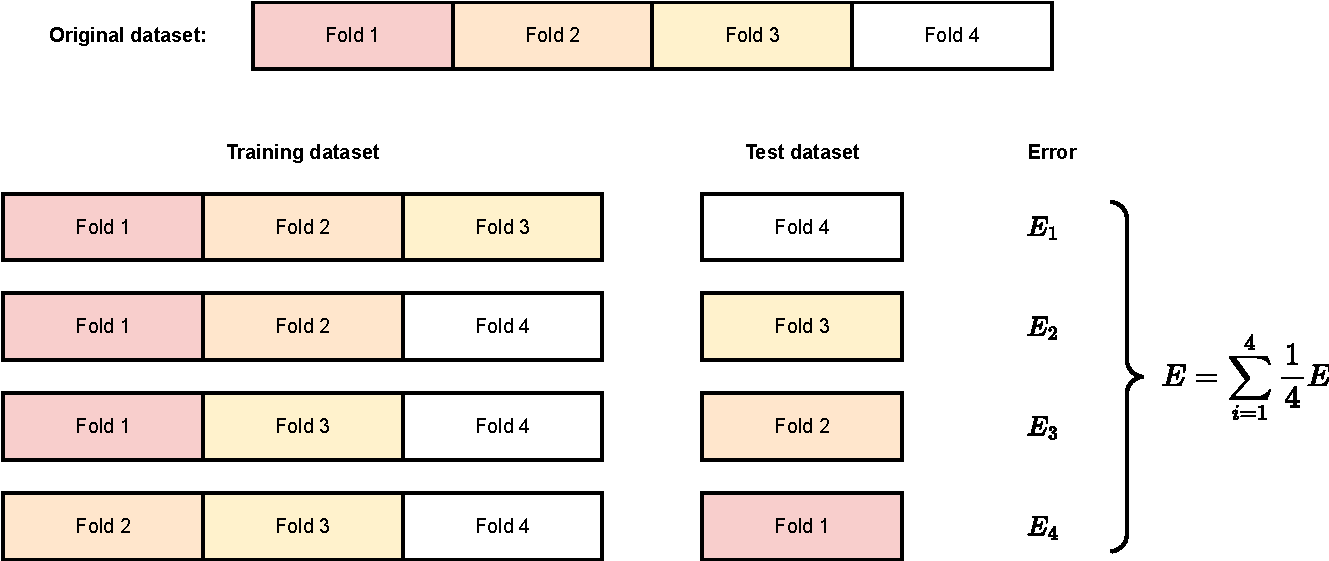
\includegraphics[width=0.8\pagewidth]{images/kfold}
		\caption{Esempio di $4$-fold cross-validation.}
	\end{figure}
	
\end{whiteframe}

\begin{frame}{Dettagli implementativi}
	
	In pratica il dataset è composto dalle matrice $\mathbf{X}$ e $\mathbf{y}$, ed ogni fold corrisponde a prendere un sottoinsieme delle loro righe.
	
	Al termine della $k$-fold cross-validation abbiamo allenato $k$ modelli diversi: in questo caso è comune allenare un ultimo modello sull'intero dataset da usare in produzione, usando $E$ come stima della sua accuracy.
	
	Una $k$-fold cross-validation dove $k$ è uguale alla dimensione del dataset viene detta \textbf{leave-one-out} (LOO) cross-validation. Maggiore $k$, migliore la stima dell'errore ma maggiore il costo computazionale.
	
\end{frame}

\subsection{Model selection}

\begin{frame}{Trovare gli iper-parametri ottimali}
	
	La maggior parte dei metodi di apprendimento richiede all'utente di selezionare uno o più iper-parametri, es.:
	%
	\begin{itemize}
		\item Il parametro $k$ nel $k$-NN.
		\item Il learning rate nella discesa al gradiente.
	\end{itemize}
	
	Supponiamo di provare diverse possibilità per ciascun iper-parametro. Come scegliamo quale sia il migliore? Sappiamo già che l'errore di allenamento è un cattivo surrogato per la capacità di generalizzazione di un modello di apprendimento. Di fatto, questi due problemi sono quasi equivalenti:
	%
	\begin{itemize}
		\item \myalert{Valutazione del modello}: valutare l'errore atteso di un modello.
		\item \myalert{Selezione del modello}: valutare l'errore atteso di due modelli per selezionare il migliore.
	\end{itemize}
	
\end{frame}

\begin{frame}{Nested cross-validation}
	
	Possiamo risolvere il problema di selezione del modello in modo equivalente al problema di valutazione del modello, ad esempio, usando un set di holdout:
	%
	\begin{enumerate}
		\item Conserviamo una parte del dataset di allenamento (chiamato \textbf{dataset di validazione}).
		\item Alleniamo diversi modelli utilizzando la parte rimanente, ognuno con una diversa scelta di iper-parametri.
		\item Selezioniamo l'iper-parametro con l'errore più basso sul dataset di validazione e ri-alleniamo il modello utilizzando l'intero dataset.
	\end{enumerate}
	
	Si può equivalentemente utilizzare holdout o k-fold cross-validation, sia per il testing che per la validazione.
	
\end{frame}

\begin{whiteframe}{Visualizzare la nested cross-validation}
	
	\vspace{1em}
	\begin{figure}
		\centering
		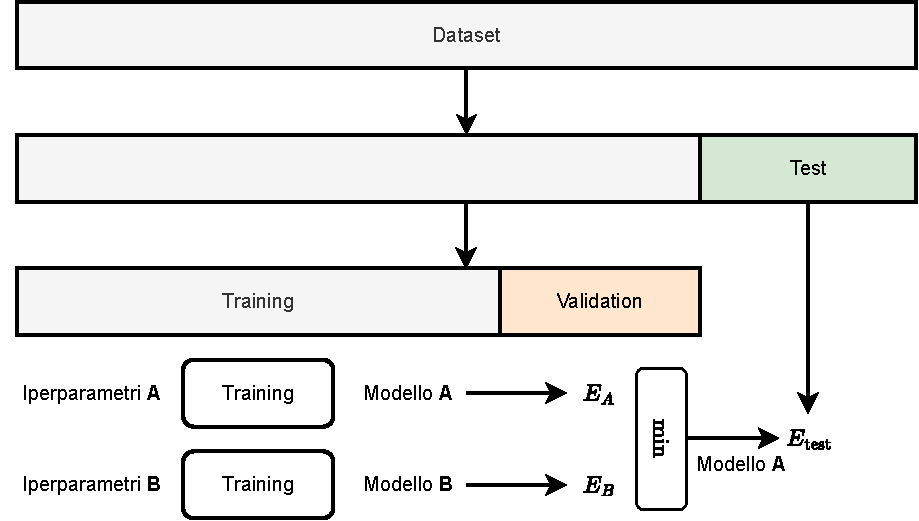
\includegraphics[width=10cm,keepaspectratio]{images/nested_validation}
		\caption{Esempio di holdout a due livelli (validazione e test). Supponiamo in questo caso di testare due set di iperparametri (A e B).}
	\end{figure}
	
\end{whiteframe}

\begin{frame}{Ricerca a griglia}
	
	Per i modelli con uno/due iper-parametri, il modo più comune per ottimizzarli è una \textbf{ricerca a griglia}, dove specificiamo un elenco di possibili configurazioni e cerchiamo in modo esaustivo quella migliore.
	
	Ad esempio, possiamo ottimizzare $k$-NN cercando $k$ in $5$, $10$, $\ldots$, $50$. Alcuni parametri sono comunemente ottimizzati in \textit{spazio logaritmico}, poiché assumiamo che piccoli cambiamenti non siano significativi.
	
	Possiamo anche ripetere diverse procedure di ricerca a griglia a diversi livelli di risoluzione, concentrandoci attorno all'ottimo della ricerca a griglia più grossolana.
	
\end{frame}

\begin{frame}{Ricerca casuale}
	
	Un'altra scelta popolare è la \textbf{ricerca casuale}:
	%
	\begin{enumerate}
		\item Specifichiamo una distribuzione di campionamento per ogni parametro, ad esempio una distribuzione uniforme in $\left[-10, 10\right]$ per $\log(C)$.
		\item Ad ogni iterazione, campioniamo casualmente una combinazione di parametri e ottimizziamo un modello fino a un certo budget di tempo computazionale.
		\item Concludiamo la ricerca dopo un dato numero di iterazioni.
	\end{enumerate}
	%
	Sia la ricerca a griglia che la ricerca casuale possano essere parallelizzate in modo banale addestrando e valutando diversi modelli contemporaneamente in un'architettura parallela.
	
\end{frame}

\begin{whiteframe}{Confronto tra ricerca a griglia e ricerca casuale}
	
	\begin{figure}
		\centering
		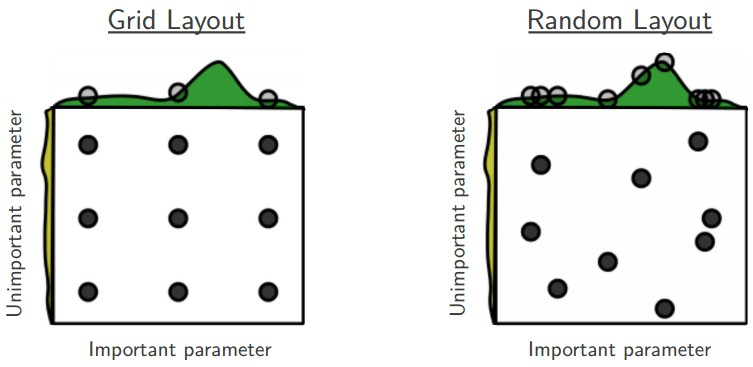
\includegraphics[width=9cm,keepaspectratio]{./images/scikitlearn8}
		\caption{\footnotesize Bergstra, J. e Bengio, Y., 2012. \textbf{Random search for hyper-parameter optimization}. \textit{Journal of Machine Learning Research}, 13(Feb), pp. 281-305.}
	\end{figure}
	
\end{whiteframe}

\begin{frame}{Selezione dell'iper-parametro come problema di ottimizzazione}
	
	Ottimizzare i parametri può essere visto come un problema di ottimizzazione; indicando con $\Theta$ l'insieme degli iper-parametri, vogliamo ottimizzare:
	%
	$$
	\Theta^* = \underset{\Theta}{\arg\min} \,\, \text{Err}(\Theta) \,,
	$$
	%
	dove $\text{Err}(\Theta)$ può essere, ad esempio, un errore validato a 5-fold sul dataset di allenamento.

	I problemi sono che (i) generalmente non possiamo calcolare alcuna derivata di $\text{Err}(\cdot)$; (ii) anche una singola valutazione della funzione obiettivo può essere costosa. \textbf{L'ottimizzazione Bayesiana} può essere utilizzata come tecnica di black-box a questo scopo.
	
\end{frame}

\subsection{Metriche per la classificazione}

\begin{frame}{Valutare un modello dopo l'allenamento}
	
	Una volta che un modello è stato allenato, dobbiamo valutarne le prestazioni. Riportare l'MSE o l'accuratezza della classificazione sul set di test è una buona misura, ma potrebbe non fornire tutte le informazioni necessarie.
	
	Come esempio concreto, consideriamo un problema di classificazione binaria, dove il $99\%$ dei dati appartiene alla classe $0$. In questo caso, un classificatore che prevede sempre $0$ come output avrebbe un'accuratezza del $99\%$! Questo è un esempio di dataset \myalert{sbilanciato}.
	
\end{frame}

\begin{frame}{Matrice di confusione}
	
	Per la classificazione binaria, gli output del classificatore possono essere raggruppati nella cosiddetta \textbf{matrice di confusione}:
	
	\def\arraystretch{1.5}
	\begin{tabular}{m{0.3\columnwidth}|m{0.3\columnwidth}|m{0.3\columnwidth}}
		& \textbf{Classe reale: $0$} & \textbf{Classe reale: $1$} \\ \hline
		\textbf{Predizione: $0$} & \cellcolor{green!20!white}TN: True negative & \cellcolor{red!20!white}FN: False negative \newline(Errore di tipo II) \\ \hline
		\textbf{Predizione: $1$} & \cellcolor{red!20!white}FP: False positive \newline(Errore di tipo I) & \cellcolor{green!20!white}TP: True positive
	\end{tabular}
	\def\arraystretch{1.0}
	
	Questo è facilmente esteso al caso multiclasse.
	
\end{frame}

\begin{frame}{Precisione e recall}
	
	Dai valori della matrice di confusione, possiamo definire diverse nuove metriche di accuratezza:
	%
	\begin{align}
		\text{Precisione} & = \frac{\text{TP}}{\text{FP} + \text{TP}} \\
		\text{Recall (o true positive rate, TPR)} & = \frac{\text{TP}}{\text{FN} + \text{TP}} \\
		\text{False positive rate} (FPR) & = \frac{\text{FP}}{\text{FP} + \text{TN}} 
	\end{align}

\end{frame}

\begin{frame}{F1-score}
	
	L'F1 score è definito come la media armonica di precisione e recall, ed è particolarmente utile in scenari sbilanciati:
	%
	\begin{equation}
		F_1 = 2 \cdot \frac{1}{\frac{1}{\text{Precisione}} + \frac{1}{\text{Recall}}} = 2 \cdot \frac{\text{Precisione} \cdot \text{Recall}}{\text{Precisione} + \text{Recall}} \,.
	\end{equation}
	%
	Intutivamente, per avere un buon F1-score, un modello deve ottimizzare allo stesso tempo sia la precision che il recall.
	
\end{frame}

\begin{frame}{Curva ROC}
	
	Nella pratica, possiamo ottenere informazioni più dettagliate sul processo di classificazione ad un livello di granularità ancora più basso, ricordando che gli output di un classificatore sono quasi sempre numeri reali, che binarizziamo per ottenere le classi finali.
	
	Fino ad ora, abbiamo considerato il caso semplice dove arrotondiamo questi output all'intero più vicino (quando $y \in \left\{0, 1\right\}$), o prendiamo il segno (quando $y \in \left\{-1, 1\right\}$). Variando effettivamente la soglia per la binarizzazione, possiamo ottenere diversi valori di recall e FPR:
	%
	\begin{itemize}
		\item Per una soglia molto bassa, otteniamo un recall perfetto (tutti i modelli sono classificati come positivi), ma un FPR molto alto.
		\item Al contrario, per una soglia molto alta, otteniamo un cattivo recall con un FPR estremamente piccolo.
	\end{itemize}
	
\end{frame}

\begin{frame}{Curva ROC (2)}
	
	Tracciando il recall contro il FPR per diverse scelte della soglia, otteniamo la cosiddetta \myalert{receiver operating curve} (ROC). L'area sotto la curva ROC (AUC) è un'altra misura molto comune di performance per un classificatore binario.
	
	Possiamo confrontare due classificatori tracciando le loro curve ROC per ottenere un set più ampio di intuizioni sul loro comportamento. Un'altra curva correlata traccia la precisione contro il recall (curva PR).
	
\end{frame}

\begin{whiteframe}{Tracciare la curva ROC}
	
	\begin{figure}
		\Wider{
			\centering
			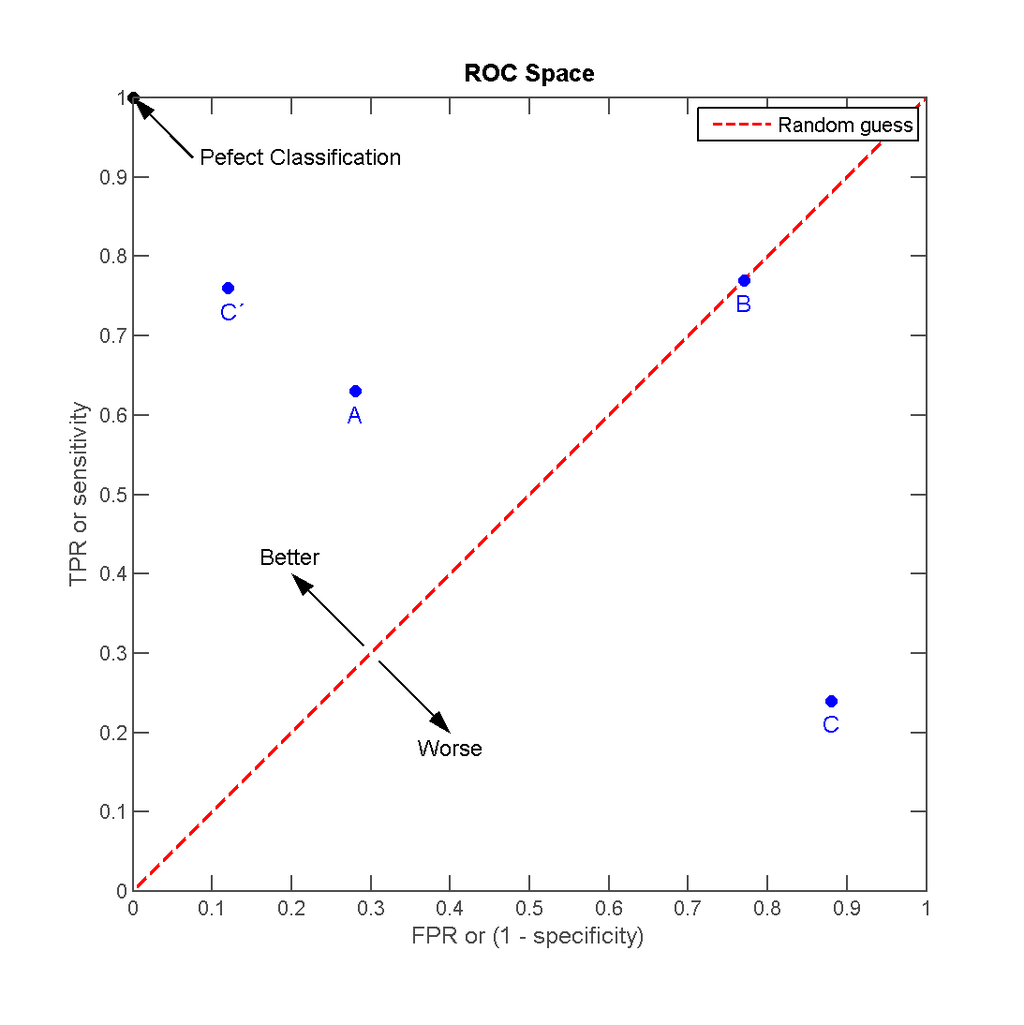
\includegraphics[width=7cm,keepaspectratio]{./images/1024px-ROC_space-2}
			\vspace{-1em}\caption{\footnotesize Se consideriamo solo una singola soglia, ogni classificatore è un punto nello spazio ROC [Wikipedia, en: Receiver Operating Characteristic].}
		}
	\end{figure}
	
\end{whiteframe}

\begin{whiteframe}{Tracciare la curva ROC (2)}
	
	\begin{figure}
		\centering
		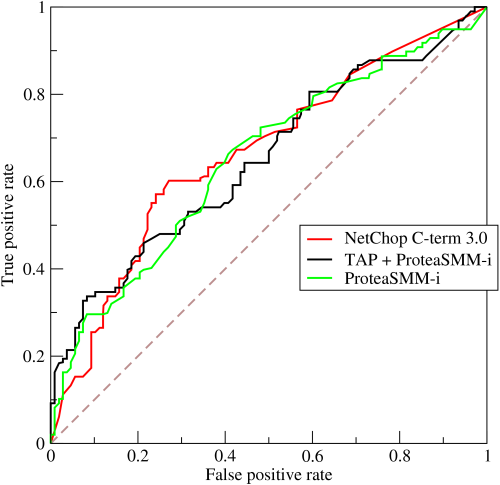
\includegraphics[width=6.5cm,keepaspectratio]{./images/Roccurves}
		\caption{\footnotesize In generale, possiamo tracciare un'intera curva nello spazio ROC [Wikipedia, en: Receiver Operating Characteristic].}
	\end{figure}
	
\end{whiteframe}

\subsection{Teoria delle decisioni}

\begin{frame}{Introduzione}
	
	Selezionare una soglia per la classificazione sulla base di un trade-off tra precision e recall è un esempio di \myalert{decision theory}.
	
	Il modello ci aiuta ad assegnare probabilità a vari eventi (es., le classi a cui assegnare $x$) ma l'effettiva decisione su quale classe scegliere può dipendere da un insieme di fattori più ampio. In questa sezione vediamo un esempio più completo basato sull'assegnazione di \textit{costi} a ciascun tipo di errore.
	
\end{frame}

\begin{frame}{Misclassification costs}
	
	Supponiamo di assegnare un \textit{costo} a ciascun elemento della matrice di confusione. Ad esempio, un falso positivo può essere valutato 10 volte peggio di un falso negativo:
	
	\begin{table}[h!]
		\centering
		\begin{tabular}{||c c c||} 
			\hline
			& Classe 1 & Classe 2 \\ [0.5ex] 
			\hline\hline
			Predizione: 1 & 0 & 10 \\ 
			Predizione: 2  & 1 & 0 \\
			\hline
		\end{tabular}
	\end{table}
	
	Idealmente, vorremmo predire la classe 1 solo se \textit{realmente} confidenti di quella predizione.
	
\end{frame}

\begin{frame}{Scelta della predizione}
	
	Supponiamo che ci siano $K$ classi. Indichiamo con $C_{ij}$ il costo di assegnare un elemento di classe $i$ alla classe $j$ (come nella tabella sopra). $f_i(x)$ è la probabilità assegnata alla classe $i$ dal nostro modello.
	
	La scelta ottimale in questo caso non è altro che la classe che minimizza il costo medio:
	%
	\begin{equation}
		c = \underset{i}{\arg\min} \;\; \sum_{j=1}^K C_{ij}f_j(x)
	\end{equation}
	
\end{frame}

\begin{whiteframe}{Un esempio visivo}
	
	\begin{figure}
			\centering
			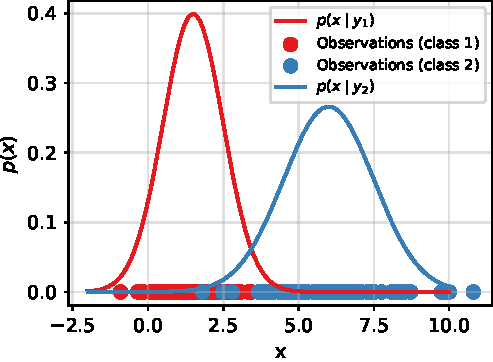
\includegraphics[width=6cm,keepaspectratio]{../scripts/decision_boundaries_1.pdf}\hspace{1em}
			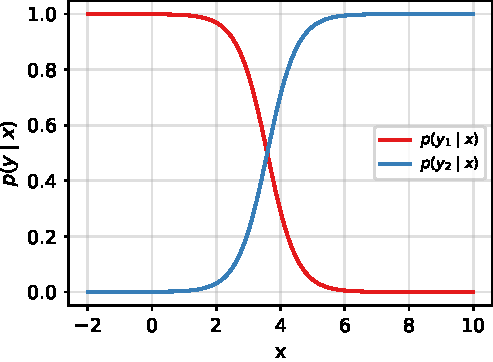
\includegraphics[width=6cm,keepaspectratio]{../scripts/decision_boundaries_2.pdf}
			\caption{Sinistra: dataset sintetico 1D. I dati per ciascuna classe sono generati da due Gaussiane (in rosso e blu). Destra: le probabilità assegnate da un modello di regressione logistica alle due classi.}
	\end{figure}
	
\end{whiteframe}


\begin{whiteframe}{Un esempio visivo (2)}
	
	\begin{figure}
		\centering
		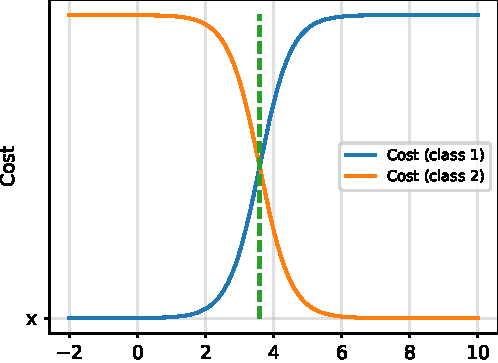
\includegraphics[width=6cm,keepaspectratio]{../scripts/decision_boundaries_3.pdf}\hspace{1em}
		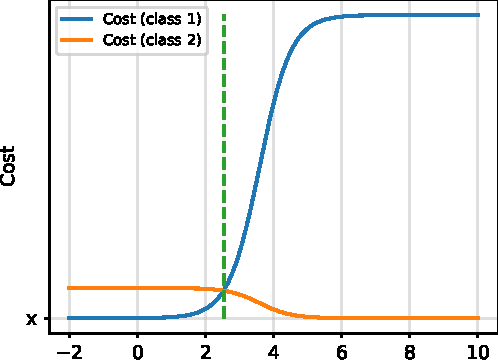
\includegraphics[width=6cm,keepaspectratio]{../scripts/decision_boundaries_4.pdf}
		\caption{Sinistra: le predizioni errate hanno costi uguali. I costi delle classi sono uguali alle probabilità assegnate dal modello. Destra: i falsi positivi `costano' 10 volte di più. In entrambi i casi scegliamo la classe con costo minore: la differenza sostanziale è nella regione `indecisa'.}
	\end{figure}
	
\end{whiteframe}

\end{document}
